\subsubsection{Overview}
\label{sec:inst_overview}

The SmartRobotinoInstructionPlanner component is responsible for the task coordination between all between various components used in the software written for the 
Robotcup Logistics League. This component was introduced by the 2016 team of Ulm University of Applied Science. The intention behind this component was that a master robot should process the information received from the Robocup Logistics Referee Box and start instructing the other robotinos on the field. Different functionalities like driving around the field or detecting some MPS stations is implemented in various components but not in the SmartRobotinoInstructionPlanner component. For instructing these components a task sequencer (which is called SmartLispServe) is used and the task or logicblocks are written in a language called SmartTCL which is based on CommonLisp //todo cite to SmartTCL. \\ 

The SmartRobotinoInstructionPlanner is connected to the RefboxServer component using two SmartSoft ports. One port is for transmitting messages from the Referee Box to the Instruction Planner and the other is for sending information about detected MPS stations back to the Referee Box. For sending information between those two components, special communication objects are used which makes it easier to parse and process those messages. These messages are based on a special DSL for communication objects which are later converted to C++ classes. With these classes those messages can be easily processed within those components. //ref to SmartSoft Communication objects. \\

The first design of the Instruction Planner was developed on the fact that when the exploration phase starts, the Referee Box sends a list of possible zones for the exploration. In these possible zones, MPS stations for the team can be located. It was intended that a master robot should process this list of zones and splits this list up into three parts. These parts can be deployed on all robotinos for exploring the field. This was the only intention of the SmartRobotinoInstructionPlanner, all other instruction logic should be implemented in the sequencer component. In 2017 the Robocup Logistics League committee removed these list of zones from the rules to make it harder for the teams to archive a successful exploration phase. Therefore the intentional implementation was now meaningless and therefore abandoned. So the meaning of the InstructionPlanner was moved more the the instruction of various components of the robotino software. \\


\subsubsection{Previous implementation}

//maybe will be discarded

As described in (reference to book of knowledge) the InstructionPlanner was designed for planning and coordination of other components on the master robotino (the one who manages the connection between the Refbox and all robotinos) but also all other robotinos. This means that it was designed that on all slave robotinos only the necessary parts like driving, detection or docking should run. All coordination should be done by the instruction planner on the master robotino. The intention behind this idea was that the referee box was sending a list of probable zone which can contain a MPS station for detection. This list of MPS stations was then splitted by an algorithm into three parts (one for each robot), so that a concurrent exploration and detection of the gamefield can be archieved. In the 2017 scenario (link to 2017 rules) this feature was discarded from the competition. In the newer scenario there is no information whether there is a MPS station or not. Therefore this feature was also discared in the new design for the 2017 competition \ref{sec:new_design}.  \\



\subsubsection{Revised design of the SmartRobotinoInstructionPlanner}
\label{sec:new_design}

As described in \ref{sec:inst_overview} the 2016 design of the Instruction Planner was discarded and a new design was created. In the 2017 design of the instruction Planner the component is now responsible for the main control of the festo robotino. The task for the team in 2017 was to implement the exploration phase for the tournament. Therefore the main responsibility for the Instruction Planner is to instruct the components of the robotino in that way that a successful exploration phase is archived.     



\subsubsection{Communication Objects Used in The InstructionPlanner}


\begin{figure}[h]
\centering
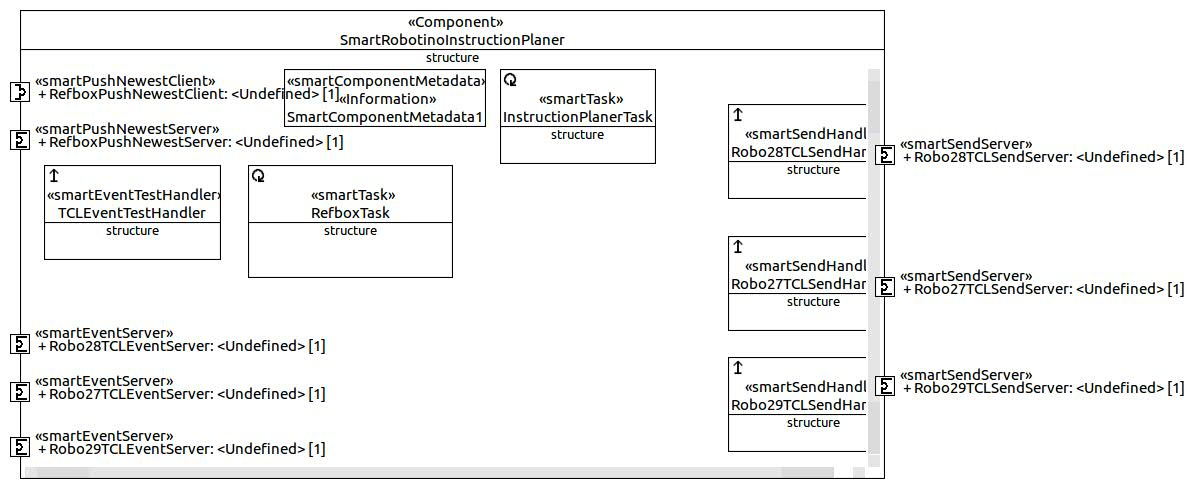
\includegraphics[scale=0.25]{pic/SmartRobotinoInstructionPlaner.JPG}
\caption{Model of InstructionPlanner}
\label{fig:i_overview}
\end{figure}


As shown in figure \ref{fig:i_overview} the SmartRobotinoInstructionPlanner has multiple input and output ports which are connected to components such as RefboxServer, MPSDetection or AlvarDetection. This connection is created over the SmartLispServer component using SmartTCL messages. On the other hand connections to the SmartLogisticsRefboxServer are done over communication objects which can be created inside smartsoft for data like the Phases, Maintenance and so on. For the connection between the Instruction Planner and the Refbox component a communication called CommRefbox is used. This object can be used to send certain data about the detected stations, exploration or production phase and the state of the robotino as seen by the 
Refereebox. \\

\newpage

Currently the CommRefbox communication object can be used to transmit the following data: 

\begin{itemize}

\item MessageType

This describes the message type. This needs to be done because in C++ the type of an object (even if we have polymorphism) can be not be derived. Therefore each message needs a message type. Valid message types are: GAMESTATE, EXPLORATION\_INFO, MACHINE\_INFO, MACHINE\_REPORT, ORDER\_INFO and 
ROBOT\_INFO. 

\item Gamestate

The gamestate part of the communication object can be used to transmit the current gamestate from the RefBoxServer to the InstructionPlanner. The elements of this submessage is the state, phase and a timestamp. 

\item ExplorationInfo (deprecated)

This was originally intended to transmit a set of zones which can include a MPS station for the team with a high probability. But because of new rules in the 2017 scenario this was dismissed. Therefore this message part is currently out of use. The explorationInfo contains a array of probable zones. 


\item machineInfos

The machineInfos message contains a list of six machineInfo which can be used as database for already detected MPS stations. The list of machineInfo begins with mInfo1 and ends with mInfo6.

\item machineInfo

The machineInfo message describes the position of a detected MPSstation with the X-Coordinate the Y-Coordinate and the orientation of the MPS-Station. This is exactly the data the Refereebox expects for a sucessfull detection of the station.


\item machineReport


The machineReport describes general information about the detected MPS stations. The informations which can be transmitted are the name of the MPS station, the zone where the MPS is localized, and the detected light signal. The lightsignal is deprecated in the 2017 scenario. 

\item robotInfo and robotState

These two message containers are used to transmit the current state of the robot as seen from the refbox. The state of the robot can be ACTIVE if everything works normal, MAINTENANCE if the team asked for a maintenance break to fix some issue of the robot or DISQUALIFIED if the robot was put into maintenance the second time or violated some rule of the contest. This message is used for internal monitoring of the contest from the robot site. For example if the robot returns from reconnects to the Referee Box from a maintenance break it can detect whether it can start to drive into the field again.  


\item orderInfo

//todo 


\end{itemize}


\subsubsection{Statemachine}


Figure \ref{fig:statemachine} shows the statemachine for the exploration phase scenario. This statemachine was implemented inside a class called RobotState. When the robotino software boots up the first state which is entered is the initial state. In this state the robot does nothing except that it waits for a signal by the referee box which triggers the EV\_EXPLORATION event. Using this event the robot knows that the exploration phase has begun and the robot can make a transition into detection state. In the detection state the robot drives around the field and tries to detect MPSstations. The detection will be done by the MPSDocking component. If this component has found a station on the field it reports this back via the LispServer component to the InstructionPlanner. If a one or more MPSstations were found the Statemachine makes a transition to the Approaching state. \\

\newpage

\begin{figure}
\centering
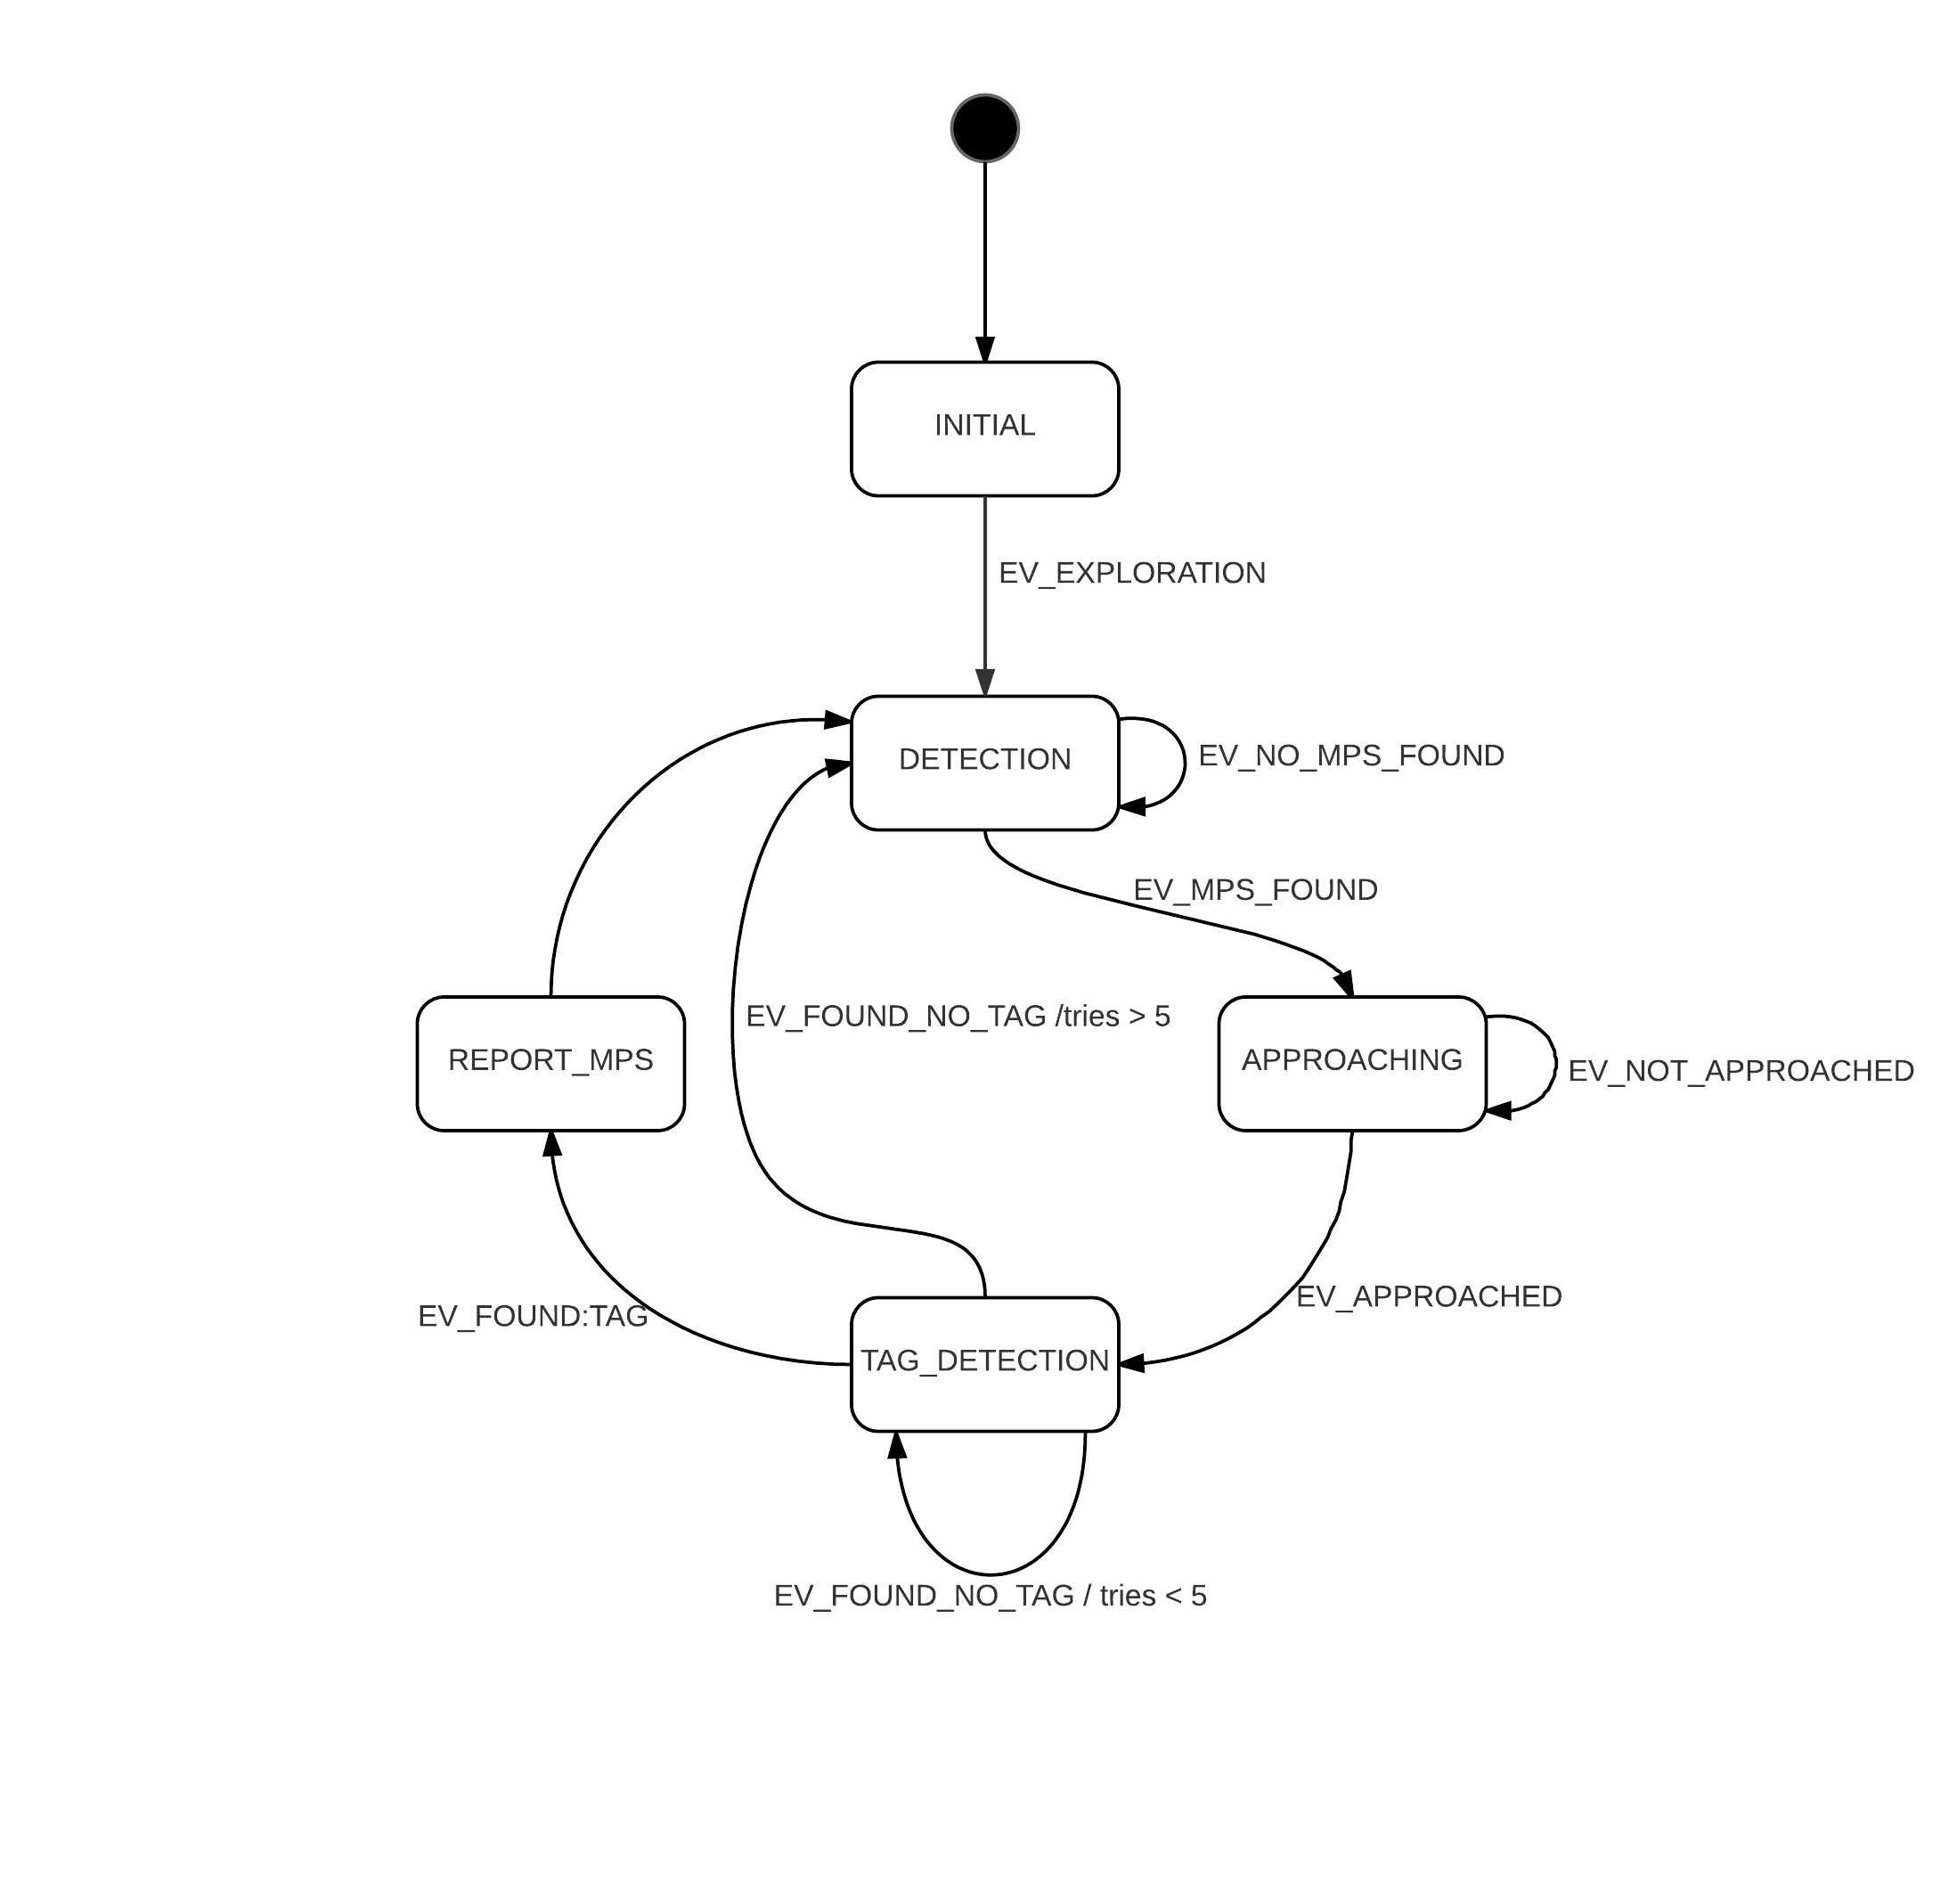
\includegraphics[scale=0.25]{pic/robotino_state_machine.png}
\caption{The statemachine for the exploration phase scenario}
\label{fig:statemachine}
\end{figure}

\newpage

In the Approaching state the robot is instructed to drive in front of the MPSstation which should later be scanned via the camera. If the robot has reached the goal (i.e. it stands in front of one of the docking points of the MPSstation) it transmits a message back which triggers the EV\_APPROACHED event. If the robot has not reached the goal (which is signaled over receiving the EV\_NOT\_APPROACHED event), the robot stays in the APPROACHING state until the goal is reached. Errorhandling is currently missing so it can be that the robotino stays in the APPROACHING state for a infinite amount of time. \\

If the approaching of the MPS was successfull the robot can start to scan the AlvarTag which is fixed on the MPSstation. This tag is used to encode the meaning or functionality of the MPS station. The scanning is instructed in the TAG\_DETECTION state. The scanning of the tag can be applied up to five times because sometimes the AlvarTag is not detected successfully. If after five tries the tag is still not detected correctly, the tag will be ignored and the robotino tries to detect new MPSstation. This is done because of the time constraints in the exploration phase. \\

If the the tag was scanned correctly it will be reported back to the Referee Box. This will be done in the REPORT\_MPS state. After this the statemachine changes into the DETECTION state. This will be done until the exploration phase is over.

\subsubsection{Advantages and Disadvantages of this design} 

\begin{itemize}

\item Advantages

For the design of the task instruction for the exploration phase, Event-driven finite-state machine was used. This pattern is often used in communication driven applications
like telecom software or communication protocols. Because the robotino software is distributed between a lot of components and these components need all to be coordinated and instructed a major component is needed which brings this all under the hood. Therefore a state machine is a good way to represent the exploration phase. The state machine is made out of states which represent certain logic blocks of the exploration phase. \\


Usually a logic block in the exploration phase is made out of a pattern:

\begin{enumerate}

\item InstructionPlanner send a message to a component.

\item The component executes some task

\item The InstructionPlanner receives a result if the task was executed sucessfully by the 
component or not.  


\end{enumerate}

For this pattern a message or event-driven state machine is really good match because the fact that a component like the AlvarTagdetection executes some logic can be designed as a state. For transition between several states the sending and receiving of messages can be used. For example to start a scan of the AlvarTag by the AlvarTagDetection component, a SmartTCL message needs to be send to the component. This induces a state transition into the state the AlvarTagDetection component is instructed to scan the tag. After the AlvarTagDetection component has finished with scanning it sends back a message which contains the tag of the MPS or a failure as the result. Using this message another state transition can be performed. \\

Because the exploration phase is made out of defined rules which the robot needs to be fulfill, this approach works well for this scenario. 


\item Disadvantages

A disadvantage is that the whole state machine needs to be handwritten by the developer because there is no tool included which can generate code out from a visual representation 
of the state machine. Although this is possible to use a seperated tool, this is not included in smart soft. Therefore if a new logic block is added to the scenario by the rcll comitee this needs to be added by hand to the state machine. This can be a very time exhausting process if the state machine contains a lot of states. Therefore another design pattern might be better here which enables adding new logic blocks in a easier way. \\

Also another big disadvantage of this design is that functionallity like this is already implemented inside the SmartSoft framework using the SmartTCL robotics behavior framework.
This framework enables it to model certain logic blocks of the exploration phase as robotic behaviors like "drive to a position" or "make a picture". The whole exploration phase can modeled using these SmartTCL task blocks. Writing these task blocks can be done using a DSL language which is implemented in Common Lisp. A disadvantage is that this Lisp based DSL is 
very different from general purpose languages like C++ or Java. But on the other side robotic tasks can be implemented easier. 


\end{itemize}


The current design is a hybrid out of SmartTCl and the event-driven finite state machine. The coordination between the components is done inside the C++ based RobotState class while the
triggering of the components is done via the Common Lisp based SmartLispServer. In the future this can be moved more to the SmartTCL implementation were the robot behavior is implemented in the SmartTCL DSL. 


\subsubsection{Maintenance Modes}

Describe how to team and the robot can react to failures and the system. How to set the robot into maintenance mode and how the robot can return to the game. 


\subsubsection{Outcome}

Multiple robots and Production phase







